
\documentclass[12pt]{article}
\setlength\parindent{0pt}
\usepackage{fullpage}
\usepackage{amsmath}
\usepackage[margin=0.5in, paperwidth=13.5in, paperheight=8.4in]{geometry}
\usepackage{graphicx}
\setlength{\parskip}{4mm}
\def\LL{\left\langle}   % left angle bracket
\def\RR{\right\rangle}  % right angle bracket
\def\LP{\left(}         % left parenthesis
\def\RP{\right)}        % right parenthesis
\def\LB{\left\{}        % left curly bracket
\def\RB{\right\}}       % right curly bracket
\def\PAR#1#2{ {{\partial #1}\over{\partial #2}} }
\def\PARTWO#1#2{ {{\partial^2 #1}\over{\partial #2}^2} }
\def\PARTWOMIX#1#2#3{ {{\partial^2 #1}\over{\partial #2 \partial #3}} }
\newcommand{\BE}{\begin{displaymath}}
\newcommand{\EE}{\end{displaymath}}
\newcommand{\BNE}{\begin{equation}}
\newcommand{\ENE}{\end{equation}}
\newcommand{\BEA}{\begin{eqnarray}}
\newcommand{\EEA}{\nonumber\end{eqnarray}}
\newcommand{\EL}{\nonumber\\}
\newcommand{\la}[1]{\label{#1}}
\newcommand{\ie}{{\em i.e.\ }}
\newcommand{\eg}{{\em e.\,g.\ }}
\newcommand{\cf}{cf.\ }
\newcommand{\etc}{etc.\ }
\newcommand{\Tr}{{\rm tr}}
\newcommand{\etal}{{\it et al.}}
\newcommand{\OL}[1]{\overline{#1}\ } % overline
\newcommand{\OLL}[1]{\overline{\overline{#1}}\ } % double overline
\newcommand{\OON}{\frac{1}{N}} % "one over N"
\newcommand{\OOX}[1]{\frac{1}{#1}} % "one over X"

\pagenumbering{gobble}

\begin{document}
\Large
\centerline{\sc{Recitation Questions}}
\normalsize
\centerline{\sc{Friday, 23 April}}


{A rock climber of mass 70 kg is climbing a cliff face when she slips and falls. She is two meters above her last anchor, so she will undergo free fall for 4 meters before the rope begins to arrest her fall. If the stiffness in her rope is 1400 N/m, then:}
  \begin{enumerate}
    \item{How far will she fall in total?}
\vspace{2in}

    \item{What is the maximum force that her rope will exert on her as it arrests her fall?}
\vspace{1.5in}

    \item When would it be desirable for a rock climber to use a rope with a large spring constant? What about a smaller spring constant? You'll need to think about 
          the engineering reasons for climbers to use ropes at all: the goal is to minimize the forces involved in arresting a climber's fall.
   \end{enumerate}

\newpage
%
% \item{A laptop battery says it has a capacity of 51 ``watt-hours''.}
%   \begin{enumerate}
%     \item{What are the dimensions of this odd unit ``watt-hour'', and what does it measure? What is 51 watt-hours in more familiar units?}
%
%\vspace{2.5in}
%
%     \item{If this battery were used to power an electric motor, how high could it lift the battery? Assume the battery has a mass of 300 grams.}
%\vspace{2.5in}
%   \end{enumerate}
%
%\newpage
 
 {A ball of mass $m$ on a cord of length $L$ is held at an angle $\theta$ to the left of the vertical and released. A very strong wind blows from left to right, exerting a constant horizontal force $F$. }

     \begin{enumerate}
       \item{Find the speed of the ball at the bottom of its swing.}
\vspace{2in}

       \item{Find an equation for the maximum angle that the ball reaches when it swings to the right. You do not need to actually solve it, since it's messy and involves a lot of trig identities; just write it down.}

\vspace{2in}

       \item{When the ball swings back to the left, find the height that it reaches. Will it come
         back to the same point where it was released? (You should be able to answer this question without doing anything difficult.)}
     \end{enumerate}


\newpage


\begin{minipage}{0.4\textwidth}
	
Mt. Wrightson is the tallest peak in the Santa Rita Mountains in southern Arizona, around 40 km north of the border with Mexico.

\bigskip
	
The usual hike up the mountain starts at around 1650 meters altitude and ends at the summit at 2850 meters.
\bigskip



Human muscles convert chemical potential energy in the food we eat into both mechanical work and heat. Depending on the type of motion, the efficiency of this motion can be as high as 25\%. Since walking is quite efficient, suppose that a hiker traveling up this mountain has an efficiency of 20\%. 

\bigskip

This means that to produce one joule of mechanical work, the hiker's metabolism must extract five joules of chemical potential energy from food; the other four joules of chemical potential energy are converted into heat (which the hiker must get rid to avoid overheating).




\end{minipage}
\hspace{0.05\textwidth}
\begin{minipage}{0.5\textwidth}
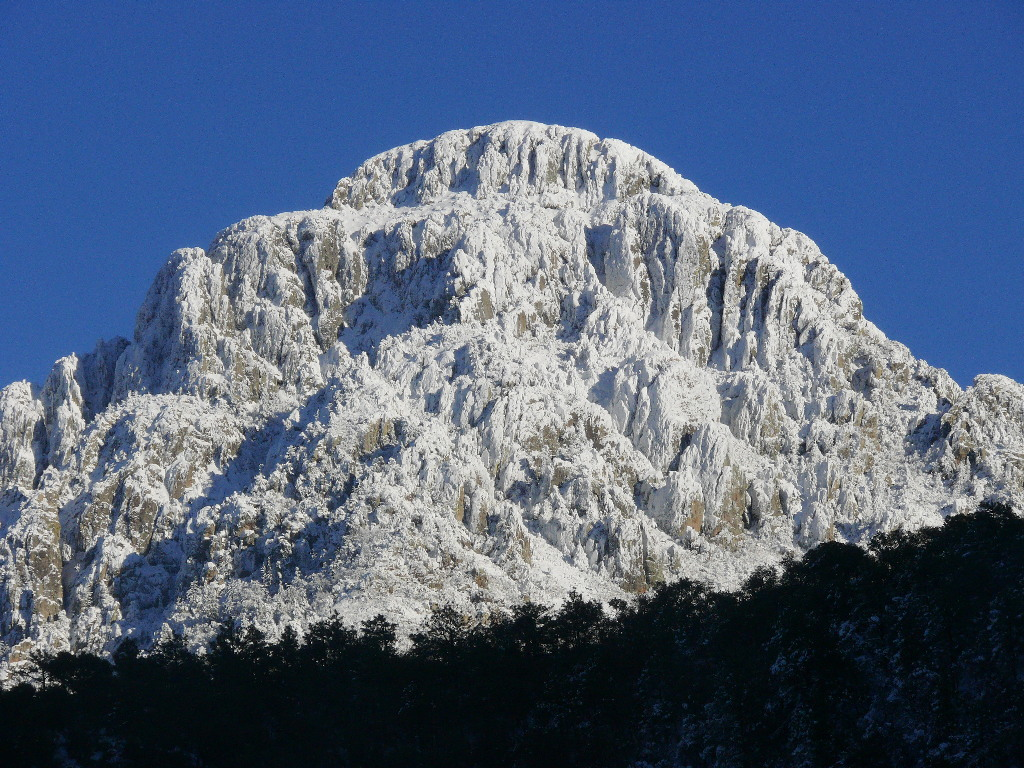
\includegraphics[width=\textwidth]{wrightson1024.jpg}
\end{minipage}


\begin{enumerate}
	\item Suppose a hiker climbs Mt. Wrightson carrying a backpack with food, water, and camping equipment. How much mechanical work must their muscles do on them for them to make it to the summit?
	\newpage
	\item How many joules of chemical potential energy must they metabolize to make this climb?
	\vspace{1in}
	\item We often measure food energy in ``kilocalories'' (or ``Calories'', with a capital letter, confusing everyone); one kcal is equal to 4180 J. How many kcal must our hiker extract from their food to make the climb?
	\vspace{1in}
	\item An apple is about 100 kcal; a Clif Bar is about 250 kcal; a big peanut butter and jelly sandwich might be 400 kcal. Is this around the amount of food you'd expect would be needed to fuel this climb?
		\vspace{1in}
		
	\item How much heat will the hiker's metabolism in the process?
	\vspace{1in}
	
	\item On a warm day, we cool ourselves during exercise mostly by evaporating sweat. The evaporation of 1 milliliter of water (with a mass of 1 gram) removes around 2500 J of heat. How much water must our hiker drink in order to make it up Mt. Wrightson?
	
\end{enumerate}


 \end{document}
